\documentclass[letterpaper, 12pt]{article}
\usepackage[francais]{babel}

\usepackage{amsmath,amsfonts,amsthm,amssymb, graphicx,wasysym,multirow}
\usepackage[latin1]{inputenc}

\pagestyle{plain}

\setlength{\topmargin}{-2cm}
\setlength{\textheight}{23.5cm}
\setlength{\textwidth}{18cm}
\setlength{\oddsidemargin}{-1cm}
\setlength{\parindent}{0pt}

%\pdfoutput=1


\begin{document}

250--  What is the horizontal axis on the Cartesian plane called?\\

a) Abscissa axis\\
b) Ordinate axis\\
c) Horizon axis\\
d) Horizontal axis\\

R\'eponse : a)\\

R\'etroaction :\\
On a Cartesian plane, the horizontal axis labels the
\emph{x}-coordinates
or \emph{abscissas }of points. Therefore, the answer is a).\\

252-- What is the name of the point of intersection of the
\emph{x}-axis
and the \emph{y}-axis on the Cartesian plane?\\

a) The center\\
b) The core\\
c) The middle point\\
d) The origin\\

R\'eponse : d)\\

R\'etroaction :\\
On a Cartesian plane, the point of intersection of the \emph{x}-axis
and
the \emph{y}-axis is called the origin. The answer is d).\\

253-- On which quadrant of the Cartesian plane are both coordinates
negative?\\

a) 1\\
b) 2 \\
c) 3\\
d) 4\\

R\'eponse : c)\\

R\'etroaction : \\
Quadrant 1 : positive abscissa, positive ordinate.\\
Quadrant 2 : negative abscissa, positive ordinate.\\
Quadrant 3 : negative abscissa, negative ordinate.\\
Quadrant 4 : positive abscissa, negative ordinate.\\

The answer is c).\\

254-- On which quadrant of the Cartesian plane are both coordinates
positive?\\

a) 1\\
b) 2 \\
c) 3\\
d) 4\\

R\'eponse : a)\\

R\'etroaction : \\
Quadrant 1 : positive abscissa, positive ordinate.\\
Quadrant 2 : negative abscissa, positive ordinate.\\
Quadrant 3 : negative abscissa, negative ordinate.\\
Quadrant 4 : positive abscissa, negative ordinate.\\

The answer is a).\\

255-- On which quadrant of the Cartesian plane is the abscissa
(\emph{x}-coordinate) negative and the ordinate
(\emph{y}-coordinate)
positive?\\

a) 1\\
b) 2 \\
c) 3\\
d) 4\\

R\'eponse : b)\\

R\'etroaction : \\
Quadrant 1 : positive abscissa, positive ordinate.\\
Quadrant 2 : negative abscissa, positive ordinate.\\
Quadrant 3 : negative abscissa, negative ordinate.\\
Quadrant 4 : positive abscissa, negative ordinate.\\

The answer is b).\\

256-- On which quadrant of the Cartesian plane is the abscissa
(\emph{x}-coordinate) positive and the ordinate
(\emph{y}-coordinate)
negative?\\

a) 1\\
b) 2 \\
c) 3\\
d) 4\\

R\'eponse : d)\\

R\'etroaction : \\
Quadrant 1 : positive abscissa, positive ordinate.\\
Quadrant 2 : negative abscissa, positive ordinate.\\
Quadrant 3 : negative abscissa, negative ordinate.\\
Quadrant 4 : positive abscissa, negative ordinate.\\

The answer is d).\\

257-- The triangle ABC has the points (2, 1), (4, 1) and
(3, 3) as vertices. It also has an axis of symmetry. What is this axis?\\

a) $x=3$\\
b) $y=3$\\
c) $x=3,5$\\
d) $y=3,5$\\

R\'eponse : a)\\

R\'etroaction : \\
The triangle ABC is isosceles. The axis of symmetry is the straight
line $x=3$ and the answer is a). Here is a plot of the triangle ABC
in the Cartesian plane.\\
    \begin{center}
    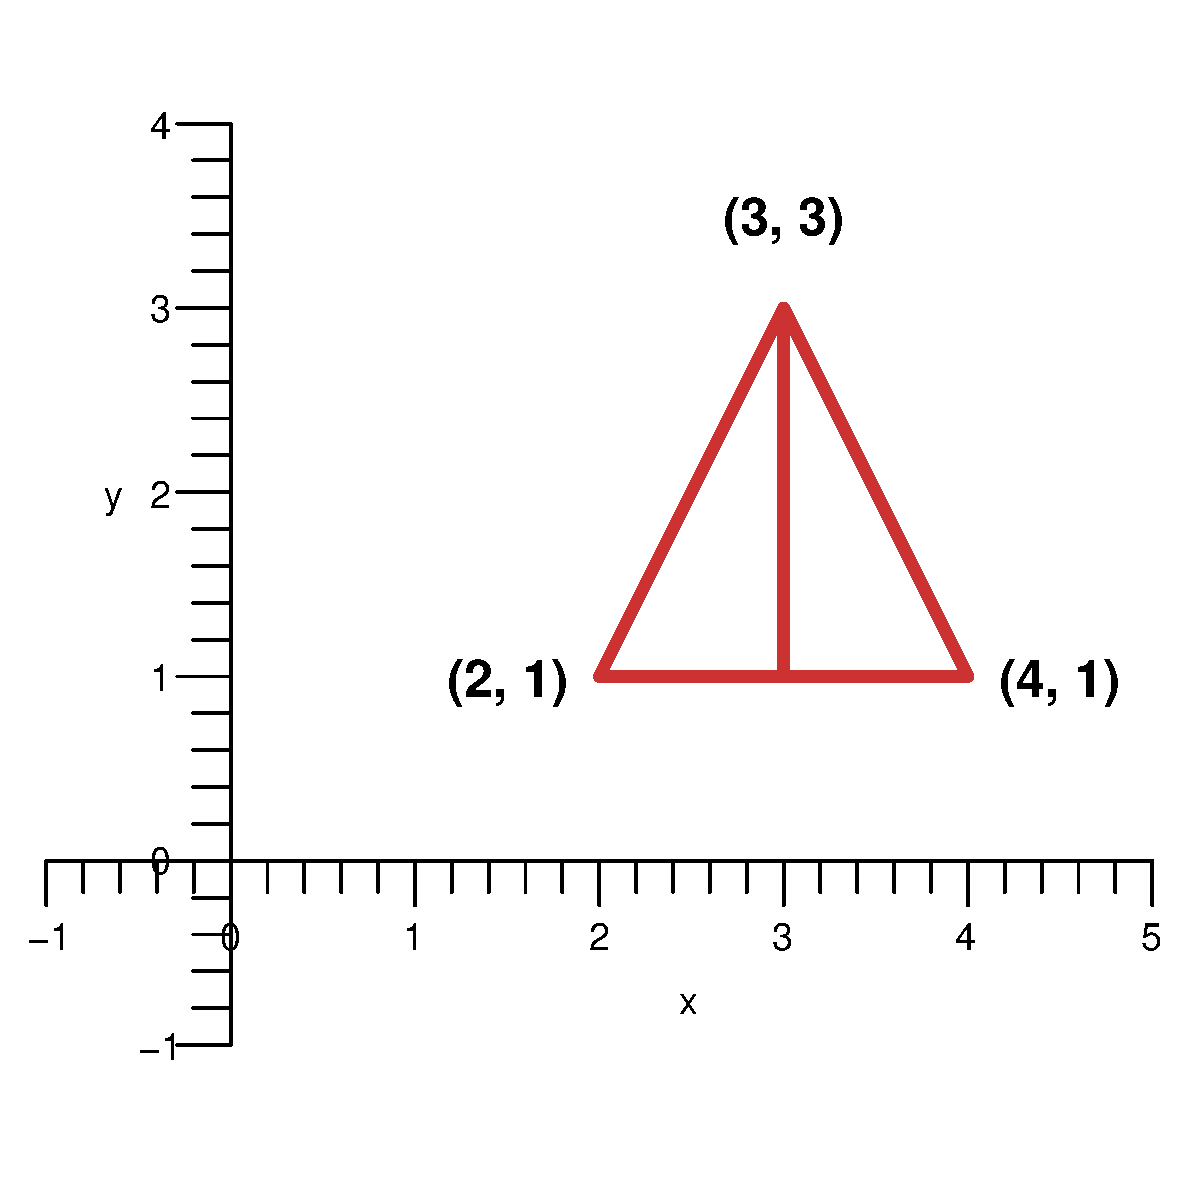
\includegraphics[width=6cm]{triangle25.eps}
% triangle25.eps : 300dpi, width=3.39cm, height=3.39cm, bb=0 0 400 400
    \end{center}


258-- Through which point of a plot does the straight line
representing a proportionality situation always pass?\\

a) (0, 0)\\
b) (1, 1)\\
c) (1, 2)\\
d) (2, 1)\\

R\'eponse : a)\\

R\'etroaction :\\
On a plot, the straight line representing a proportionality
situation always passes through the origin, i.e. the point (0, 0).
The answer is a).\\

259-- Out of the following choices, which pair of elements is
sufficient to fully define an homothety?\\

a) The center and the length.\\
b) The center and the ratio.\\
c) The middle point and the length.\\
d) The middle point and the ratio.\\

R\'eponse : b)\\

R\'etroaction :\\
The center and the ratio of an homothety are needed to fully define
it. The answer is b). \\

260-- Out of the following choices, which pair of elements is
sufficient to fully define an homothety?\\

a) The center and two image points.\\
b) The center and any two points.\\
c) The center, a point, and the image of that point.\\
d) A point and its image.\\

R\'eponse : c)\\

R\'etroaction :\\
A center, a point, and the image of that point are necessary to
fully define an homothety. The homothety ratio and the image of
every point can be found from these three elements. The correct answer is c).\\


262-- Which statement is true?\\

a) A homothety maps a straight line into a straight line that overlaps it.\\
b) A homothety maps a straight line into a parallel straight line.\\
c) A homothety maps a straight line into a perpendicular straight
line.\\
d) A homothety maps a straight line a into a secant straight line.\\

R\'eponse : b)\\

R\'etroaction : \\
A homothety maps a straight line into a parallel straight line. The
answer is b).\\

263--  Which statement is true?\\

a) In a homothety, the angles are transformed according to the
homothety ratio.\\
b) In a homothety, the angles are transformed according to the
inverse of the homothety ratio.\\
c) The sizes of angles are invariant under homotheties.\\
d) The sizes of angles are not invariant under homotheties.\\

R\'eponse : c)\\

R\'etroaction :\\
The sizes of angles are invariant under homotheties. The correct
answer is c). \\

264-- Which statement is true?\\

a) Homotheties map line segments into line segments of
proportional lengths.\\
b) Homotheties map line segments into line segments of
non-proportional lengths.\\
c) Homotheties map line segments into line segments of smaller
lengths.\\
d) Homotheties map line segments into line segments of larger
lengths.\\

R\'eponse : a)\\

R\'etroaction :\\
Homotheties map line segments into line segments of proportional
lengths. The answer is a).\\

265-- Which statement is true?\\

a) In a homothety, a negative ratio means that the image figure is
missing sides.\\
b) In a homothety, a negative ratio means that the image figure is
smaller.\\
c) In a homothety, a negative ratio means that the initial figure
and the image figure are located on different sides of the homothety
center.\\
d) In a homothety, a negative ratio means that the initial figure
and the image figure are located on the same side of the homothety
center.\\

R\'eponse : c)\\

R\'etroaction : \\
In a homothety, a negative ratio means that the initial figure and
the image figure are located on different sides of the homothety
center. The answer is c).\\


266-- In a skill game, Preci Sion must throw a ball into a water
bucket in such a way that it touches the bottom. Bucket A is 1.7 m
away from him and contains water at $-5^{\circ}$C. Bucket B is 0.5 m
away from him and contains water at $-2^{\circ}$C. Bucket C is 2 m
away from him and contains water at $2^{\circ}$C. Finally, Bucket B
is 1.5 m away from him and contains water at $-4^{\circ}$C.  What
Bucket must Preci
Sion aim at to have the best chances to win?\\

a) Bucket A\\
b) Bucket B\\
c) Bucket C\\
d) Bucket D\\

R\'eponse : c)\\

R\'etroaction : \\
If Precis Ion aims at Bucket A, B, C, or D, the ball will never
touch the bottom because the water they contain is frozen. The
answer is c).\\

267-- Out of the following daily situations, which one represents a
situation where a homothety with a negative ratio is applied?\\

a) The way the human eye works.\\
b) The motion of a bicycle pedal.\\
c) Someone riding a bicycle.\\
d) Someone looking in a mirror.\\

R\'eponse : a)\\

R\'etroaction : \\
Someone looking in the mirror is suggestive of a reflection. Someone
riding a bicycle evokes a translation because he is moving
horizontally. A bicycle pedal makes a rotation motion because it
moves around an axis. The way the human eye works evokes a homothety
with a negative ratio because the image projected on the retina is
the inverse image of what is actually seen. The correct answer is a).\\

268-- A quadrilateral whose sides measure 4.2 \, cm, 3.4 \,cm, 2.25
\,cm, and 3.1 \,cm is subjected to a homothety of ratio $-2$.
What are the new lengths of its sides?\\

a) $-8.4$\,cm, $-6.8$\,cm, $-4.5$\,cm, $-6.2$\,cm\\
c) 2.2\,cm, 1.4\,cm, 0.5\,cm, 1.1\,cm\\
b) 2.1\,cm, 1.7\,cm, 1.125\,cm, 1.55\,cm\\
d) 8.4\,cm, 6.8\,cm, 4.5\,cm, 6.2\,cm\\

R\'eponse : d)\\

R\'etroaction : \\
With a $-2$ ratio, the transformed figure will be twice as large as
the initial figure, but it will not be located on the same side of
the center. The answer is d). \\

269-- Which statement is true?\\

a) In a homothety, the transformed figure is smaller than the
initial figure only when the homothety ratio is between $-1$ and 0.\\
b) In a homothety, the transformed figure is smaller than the
initial figure only when the homothety ratio is between 0 and $1$.\\
c) In a homothety, the transformed figure is smaller than the
initial figure only when the homothety ratio is between $-1$ and 0 or 0 and $1$.\\
d) In a homothety, the transformed figure is smaller than the
initial figure only when the homothety ratio is negative.\\

R\'eponse : c)\\

R\'etroaction : \\
In a homothety, the transformed figure is smaller than the initial
figure only when the homothety ratio is between $-1$ and 0 or 0 and
$1$.
Therefore, the answer is c).\\

270-- Which statement about homotheties is true?\\

a) When the homothety ratio is $-1$ or 1, the final figure is an
exact reproduction of the initial figure.\\
b) When the homothety ratio is 0, the final figure is an
exact reproduction of the initial figure.\\
c) When the homothety ratio is 1, the final figure is not an exact
reproduction of the initial figure.\\
d) When the homothety ratio is 0 or 1, the final figure is an exact
reproduction of the initial figure.\\

R\'eponse : a)\\

R\'etroaction : \\
When the homothety ratio is $-1$ or 1, the final figure is an exact
reproduction of the initial figure. The correct answer is a).\\


272-- Which of the following factor represents an enlargement in an
homothety?\\

a) 45$\,\%$\\[2mm]
b) $\frac{7}{8}$\\[2mm]
c) $\frac{8}{7}$\\[2mm]
d) 0.66\\

R\'eponse : c)\\

R\'etroaction :\\
To have an enlargement, the homothety ratio must be larger than 1 or
smaller than $-1$.\\[2mm]
45$\,\%$ = 0.45 is a number between 0 and 1.\\[2mm]
$\frac{7}{8}$ is a fraction between 0 and 1.\\[2mm]
$\frac{8}{7}$ is a fraction larger than 1.\\[2mm]
0.66 is a decimal number between 0 and 1.\\[2mm]
The correct answer is c).\\

273-- Which of the following homothety ratio corresponds to a
reduction?\\

a) $-1.1$\\[2mm]
b) 110$\,\%$\\[2mm]
c) 0.25\\[2mm]
d) $\frac{9}{7}$\\

R\'eponse : c)\\

R\'etroaction : \\
To have a reduction, the homothety ratio must be between $-1$
and 0 or between 0 and 1.\\[2mm]
$-1.1$ is smaller than $-1$.\\[2mm]
110$\,\%$ is larger than 1.\\[2mm]
0.25 is between 0 and 1\\[2mm]
$\frac{9}{7}$ is larger than 1.\\[2mm]
The answer is c).\\

274-- A quadrilateral has sizes with lengths 4.3 \,cm, 2.15 \,cm,
7.4 \,cm, and 3.1 \,cm. After a particular homothety, the lengths of
the sizes change to 12.9 \,cm, 6.45 \,cm, 22.2 \,cm et 9.3 \,cm
respectively. Out of the following choices, which one represents all
the possible values of the homothety ratio?\\

a) $\frac{-1}{3}$ or $\frac{1}{3}$ \\[2mm]
b) $-3$ or 3 \\[2mm]
c) $\frac{1}{3}$\\[2mm]
d) 3 \\

R\'eponse : b)\\

R\'etroaction : \\
The final figure is larger than the initial figure. Therefore, the
homothety ratio has to be an enlargement factor. In other words, it
has to be larger than 1 or smaller than $-1$. Since whether or not
the two figures lie on the same side of the homothety center is not
stated in the question, the sign of the homothety ratio remains
unknown. Therefore, the answer is b).\\

275-- An initial figure labeled \emph{F1} is subjected to an
homothety of ratio 2. This figure labeled \emph{F2} is then
subjected to an homothety
of ratio 3 to become F3. What is the homothety ratio from \emph{F1} to \emph{F3}?\\

a) $-6$\\
b) 1\\
c) 5\\
d) 6\\

R\'eponse : d)\\

R\'etroaction : \\
This problem deals with a composition of homotheties. After the
first transformation, the figure \emph{F2} is twice as large as
\emph{F1}. Since \emph{F2} is subjected to an homothety of ratio 3
to become \emph{F3}, figure \emph{F3} is three times larger than
\emph{F2}, or six times larger than \emph{F1}. One simply needs to
take the product of the two homothety ratios. Therefore, the
answer is d).\\

276-- A figure labeled \emph{F1} is subjected to an homothety of
ratio 1.8. The figure obtained labeled \emph{F2} is than subjected
to a reduction of factor 0.5, transforming into a third figure
labeled \emph{F3}. What is the homothety ratio from \emph{F1} to \emph{F3}?\\

a) 0.9\\
b) 1.3\\
c) 2.3\\
d) 3.6\\

R\'eponse : a)\\

R\'etroaction : \\
This problem deals with a composition of homotheties. After the
first homothety, the figure \emph{F2} is 1.8 times larger than
\emph{F1}. Figure \emph{F3} is twice as small as \emph{F2} because
it has been subjected to an homothety of ratio 0.5. Simple
arithmetic tells us that the
homothety ratio from \emph{F1} to \emph{F3} is 0.9. The answer is a).\\

277-- A rectangle measuring 1.9 \,m by 2.7 \,m is subjected to an
homothety of ratio 1.2. The image obtained is then subjected to an
homothety of ratio 0.7. What is the size of the figure obtained
after this second homothety?\\


a) 0.95\,m by 1.35\,m\\
b) 1.33\,m by 1.89\,m\\
c) 1.596\,m by 2.268\,m\\
d) 3.612\,m by 5.154\,m\\

R\'eponse : c)\\

R\'etroaction : \\
After the homothety of ratio 1.2, the size of the rectangle is
2.28\,m by 3.24\,m.\\
$1.9$\,m $\times\,1.2=2.28$\,m\\
$2.7$\,m $\times\,1.2=3.24$\,m\\
This transformed rectangle is subjected to an homothety of ratio
0.7\\
$2.28$\,m $\times\,0.7=1.596$\,m\\
$3.24$\,m $\times\,0.7=2.268$\,m\\
The size of the final rectangle is 1.596\,m by 2.268\,m.\\
The answer is c).\\

278-- A rectangle of size 12 \,cm by 18 \,cm is subjected to an
homothety of ratio $\frac{1}{2}.$ What is the ratio of the area of
the final rectangle to the area of the initial rectangle?\\

a) $\frac{1}{8}$\\[2mm]
b) $\frac{1}{4}$\\[2mm]
c) $\frac{1}{2}$\\[2mm]
d) 2\\

R\'eponse : b)\\

R\'etroaction : \\
The area of the initial rectangle is 216\,cm$^{2}$.  After the
homothety, its size is 6\,cm par 9\,cm and its area is 54\,cm$^{2}$.
The ratio of the final to the initial area is
$\frac{54}{216}=\frac{1}{4}.$  Therefore, the answer is b).\\

279-- Which statement is true?\\

a) The size of the corresponding angles of two similar figures is
inversely proportional to the size of the sides.\\
b) The size of the corresponding angles of two similar figures are
proportional to the size of the sides.\\
c) The corresponding angles of two similar figures don't have the same size.\\
d) The corresponding angles of two similar figures have the same size.\\

R\'eponse : d)\\

R\'etroaction : \\
The corresponding angles of two similar figures have the same size.
The answer is d).\\

280-- Which statement is true?\\

a) All the regular pentagons are similar.\\
b) All the rectangles are similar.\\
c) All the isosceles triangles are similar.\\
d) All the right triangles are similar.\\

R\'eponse : a)\\

R\'etroaction : \\
Rectangles are not all similar. For example, the two following
rectangles are not similar.\\
    \begin{center}
    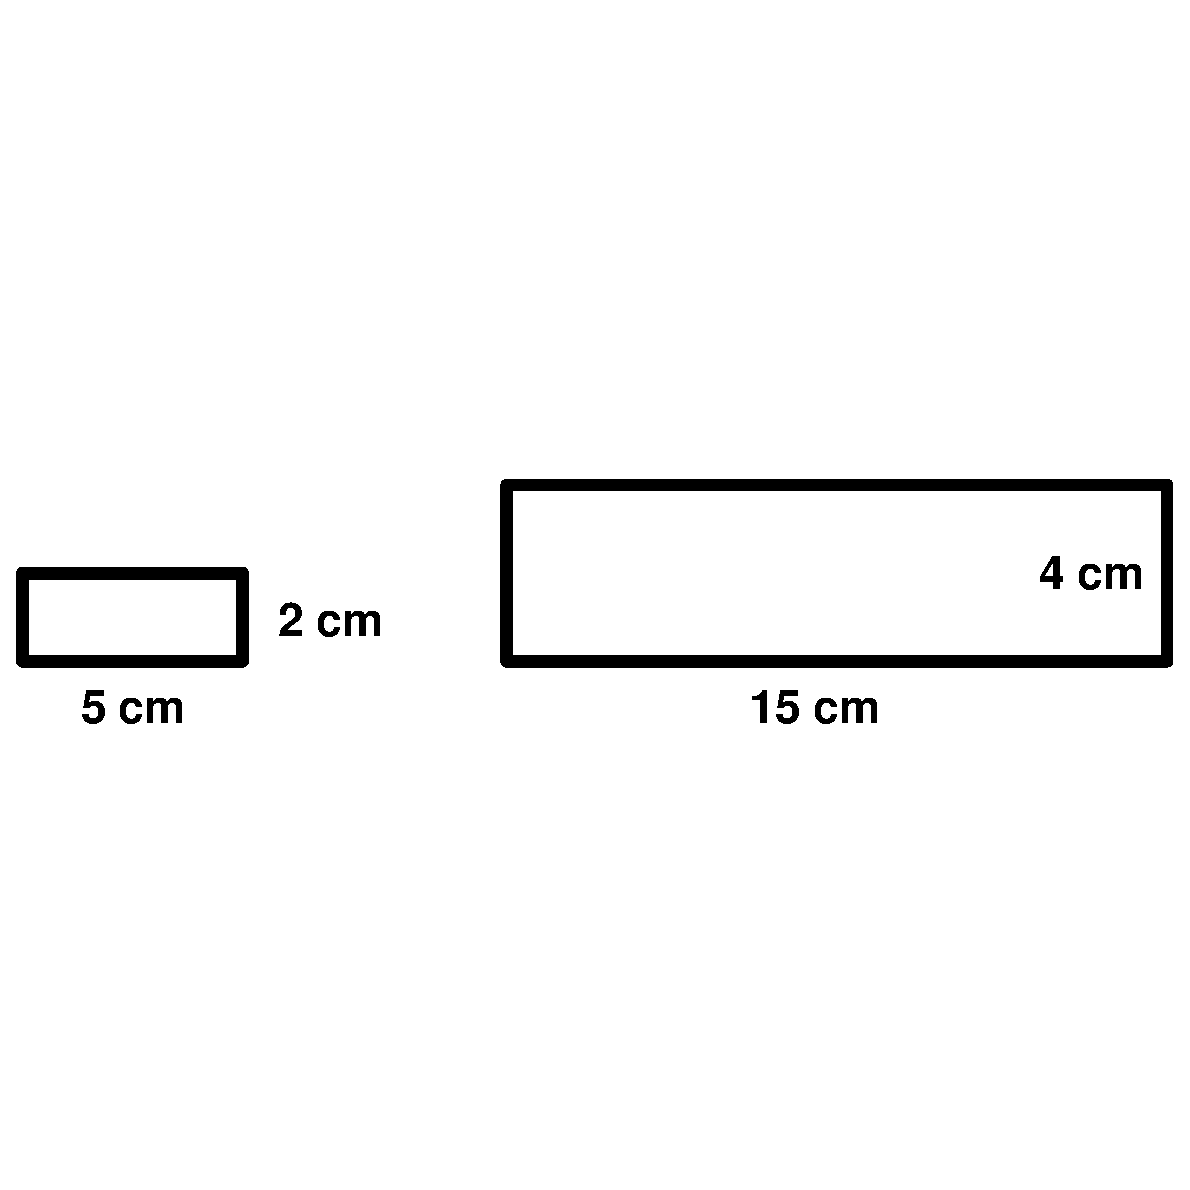
\includegraphics[width=6cm]{rectanglesemblable1.eps}
% rectanglesemblable.eps : 300dpi, width=3.39cm, height=3.39cm, bb=0 0 400 400
    \end{center}

Right triangles are not all similar. For example, the following two
right triangles are not similar.
    \begin{center}
    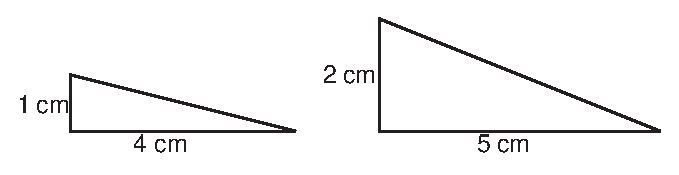
\includegraphics[width=7cm]{trianglesemblable.eps}
% trianglesemblable.eps : 300dpi, width=3.39cm, height=3.39cm, bb=0 0 400 400
    \end{center}

Isosceles triangles are not all similar. For example, the following
two isosceles triangles are not similar.
    \begin{center}
    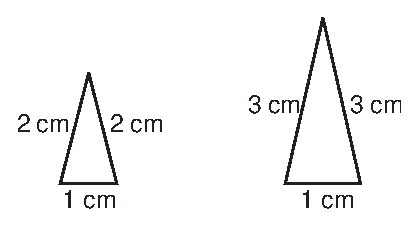
\includegraphics[width=6cm]{trianglesemblable1.eps}
% trianglesemblable1.eps : 300dpi, width=3.39cm, height=3.39cm, bb=0 0 400 400
    \end{center}
By definition, the 5 sides of a regular pentagon all have the same
size. Therefore, if the length of one side is changed, the lengths
of all the other sides must also change for the pentagon to remain
regular.
All the regular pentagons are similar.\\
The answer is a).\\



282-- The vertices of the triangle ABC have the following
coordinates on the Cartesian plane : (3,\,2), (5,\,7) et (1,\,1). If
it is subjected to the translation $t_{\left( a,\,b\right) } :\left(
x,\,y\right) \longmapsto \left(x+4,\,y-2\right) $, what are the new
coordinates its vertices?\\

a) (1, 6), (3, 11) et (--1, 5)\\
b) (0, 7), (5, 9) et (--1, 5)\\
c) (7, 0), (9, 5) et (5, --1)\\
d) (6, 4), (10, 14) et (2, 2)\\

R\'eponse : c)\\

R\'etroaction : \\
One must add 4 to each $x$-ccordinate and 2 to each $y$-coordinate.
The answer is c).\\


283-- On a Cartesian plane, the point (4, 6) has been mapped to
($-5$, 12) after being subjected to a translation. Which of the
following represents the translation rule that was used?\\

a) $t_{\left( a,\,b\right) } :\left( x,\,y\right) \longmapsto
\left(x-9,\,y-6\right) $\\
b) $t_{\left( a,\,b\right) } :\left(x,\,y\right)\longmapsto
\left(x+9,\,y+6\right)$\\
c) $t_{\left( a,\,b\right) } :\left(x,\,y\right )\longmapsto
\left(x+6,\,y-9\right)$\\
d) $t_{\left( a,\,b\right) } :\left(x,\,y\right)\longmapsto
\left(x-9,\,y+6\right)$\\

R\'eponse : d)\\

R\'etroaction :\\
To find the translation rule, one must substract the intial form the
final coordinates.\\
For the $x$-coordinate :  -5-4=$-9$\\
For the $y$-coordinate :  12-6=6\\
The translation is represented by $t_{\left( a,\,b\right) }
:\left(x,\,y\right)\longmapsto \left(x-9,\,y+6\right)$.
Therefore, the answer is d).\\

284-- A translation in the Cartesian plane is defined by the rule
$t_{\left( a,\,b\right) } :\left(x,\,y\right)\longmapsto
\left(x+a,\,y+b\right) $ and the image of the origin is in the first
quadrant. Which answer choice gives the possible values of $a$
and $b$?\\

a) $a<0$ and $b<0$\\
b) $a<0$ and $b>0$\\
c) $a>0$ and $b<0$\\
d) $a>0$ and $b>0$\\

R\'eponse : d)\\

R\'etroaction : \\
In the first quadrant, the $x$-coordinates and the $y$-coordinates
are positive. The answer is d).\\

285-- A translation in the Cartesian plane is defined by the rule
$t_{\left( a,\,b\right) } :\left(x,\,y\right)\longmapsto
\left(x+a,\,y+b\right) $ and the image of the origin is in the
second quadrant. Which answer choice represents possible values for $a$ and $b$?\\

a) $a<0$ and $b<0$\\
b) $a<0$ and $b>0$\\
c) $a>0$ and $b<0$\\
d) $a>0$ and $b>0$\\

R\'eponse : b)\\

R\'etroaction : \\
In the second quadrant, the $x$-coordinates are negative and the
$y$-coordinates are positive. We need $a<0$ and $b>0$. The answer is
b).\\

286-- A translation on the Cartesian plane is defined by the rule
$t_{\left( a,\,b\right) } :\left(x,\,y\right)\longmapsto
\left(x+a,\,y+b\right) $ and the image of the origin is in the third
quadrant. Which answer choice represent possible values for $a$ and $b$?\\

a) $a<0$ and $b<0$\\
b) $a<0$ and $b>0$\\
c) $a>0$ and $b<0$\\
d) $a>0$ and $b>0$\\

R\'eponse : a)\\

R\'etroaction : \\
In the third quadrant, $x$-coordinates and the $y$-coordinates are
negative. We need $a<0$ and $b<0$. The answer is a).\\

287-- A translation in the Cartesian plane is represented by the
rule $t_{\left( a,\,b\right) } :\left(x,\,y\right)\longmapsto
\left(x+a,\,y+b\right) $ and the image of the origin is in the
fourth quadrant. Which answer choice represents possible values for
$a$ and $b$?\\

a) $a<0$ et $b<0$\\
b) $a<0$ et $b>0$\\
c) $a>0$ et $b<0$\\
d) $a>0$ et $b>0$\\

R\'eponse : c) \\

R\'etroaction : \\
In the fourth quadrant, the $x$-coordinates are positive and the
$y$-coordinates are negative. We need $a>0$ and $b<0$. The answer
is c).\\

288-- Which answer choice represents the rule of a vertical
translation in a Cartesian plane?\\

a) $t_{\left( a,\,b\right) } :\left(x,\,y\right)\longmapsto
\left(x,\,y+b\right) $\\
b) $t_{\left( a,\,b\right) } :\left(x,\,y\right)\longmapsto
\left(x+a,\,y\right) $\\
c) $t_{\left( a,\,b\right) } :\left(x,\,y\right)\longmapsto
\left(x+a,\,y+b\right) $\\
d) $t_{\left( a,\,b\right) } :\left(x,\,y\right)\longmapsto
\left(x+b,\,y+b\right) $\\

R\'eponse : a)\\

R\'etroaction :\\
In a vertical translation, the $x$-coordinate remains unchanged and
the $y$-coordinate is modified. Therefore, the answer is a).\\

289-- Which answer choice corresponds to the rule of a horizontal
translation on a Cartesian plane?\\

a) $t_{\left( a,\,b\right) } :\left(x,\,y\right)\longmapsto
\left(x,\,y+b\right) $\\
b) $t_{\left( a,\,b\right) } :\left(x,\,y\right)\longmapsto
\left(x+a,\,y\right) $\\
c) $t_{\left( a,\,b\right) } :\left(x,\,y\right)\longmapsto
\left(x+a,\,y+b\right) $\\
d) $t_{\left( a,\,b\right) } :\left(x,\,y\right)\longmapsto
\left(x+b,\,y+b\right) $\\

R\'eponse : b)\\

R\'etroaction :\\
In a horizontal translation, the $x$-coordinate is modified and the
$y$-coordinate remains unchanged. Therefore, the answer is b).\\

290-- Which answer represents a 180$^{\circ}$ rotation in the Cartesian plane?\\

a) $r_{\left( 0,\,180^{\circ}\right) } :\left( x,\,y\right)
\longmapsto
\left(-x,\,-y\right) $ \\
b) $r_{\left( 0,\,180^{\circ}\right) } :\left( x,\,y\right)
\longmapsto
\left(-y,\,-x\right) $ \\
c) $r_{\left( 0,\,180^{\circ}\right) } :\left( x,\,y\right)
\longmapsto
\left(y,\,-x\right) $\\
d) $r_{\left( 0,\,180^{\circ}\right) } :\left( x,\,y\right)
\longmapsto
\left(-x,\,y\right) $\\

R\'eponse : a)\\

R\'etroaction : \\
The rule of a 180$^{\circ}$ rotation is $r_{\left(
0,\,180^{\circ}\right) } :\left( x,\,y\right) \longmapsto
\left(-x,\,-y\right) $.\\
To get a 180$^{\circ}$ rotation, one simply needs to change the sign
of each coordinate. The answer is a).\\

291-- Which answer choice represents the rule of a 90$^{\circ}$ rotation in a Cartesian plane?\\

a) $r_{\left( 0,\,90^{\circ}\right) } :\left( x,\,y\right)
\longmapsto
\left(-x,\,-y\right) $ \\
b) $r_{\left( 0,\,90^{\circ}\right) } :\left( x,\,y\right)
\longmapsto
\left(-y,\,-x\right) $ \\
c) $r_{\left( 0,\,90^{\circ}\right) } :\left( x,\,y\right)
\longmapsto
\left(-y,\,x\right) $\\
d) $r_{\left( 0,\,90^{\circ}\right) } :\left( x,\,y\right)
\longmapsto
\left(-x,\,y\right) $\\

R\'eponse : c)\\

R\'etroaction : \\
The rule of a 90$^{\circ}$ rotation is $r_{\left(
0,\,90^{\circ}\right) } :\left( x,\,y\right) \longmapsto
\left(-y,\,x\right)
$. The answer is c).\\

292-- Which answer choice represents the rule of a  $-90^{\circ}$ rotation in the Cartesian plane?\\

a) $r_{\left( 0,\,-90^{\circ}\right) } :\left( x,\,y\right)
\longmapsto
\left(-x,\,-y\right) $ \\
b) $r_{\left( 0,\,-90^{\circ}\right) } :\left( x,\,y\right)
\longmapsto
\left( y,\,-x\right) $ \\
c) $r_{\left( 0,\,-90^{\circ}\right) } :\left( x,\,y\right)
\longmapsto
\left(-y,\,x\right) $\\
d) $r_{\left( 0,\,-90^{\circ}\right) } :\left( x,\,y\right)
\longmapsto
\left(-x,\,y\right) $\\

R\'eponse : b)\\

R\'etroaction : \\
The rule of a $-90^{\circ}$ rotation is $r_{\left(
0,\,-90^{\circ}\right) } :\left( x,\,y\right) \longmapsto \left(
y,\,-x\right) $.  The answer is b).\\

293-- The coordinates of a point on the Cartesian plane are (5, 7).
It is then mapped to the point (7, --5). What kind of transformation
has it been subjected to?\\

a) A reflection with respect to the $x$-axis.\\
b) A reflection with respect to the $y$-axis.\\
c) A $-90^{\circ}$ rotation.\\
d) A $90^{\circ}$ rotation.\\

R\'eponse : c)\\

R\'etroaction : \\
The point $(x,\,y)$ has become $(y,\,-x)$. This is a
$-90^{\circ}$ rotation. Therefore, the answer is c).  \\

294-- Which answer choice corresponds to the rule of a reflection
with respect to the $x$-axis on the Cartesian plane?\\

a) $s_x :\left( x,\,y\right) \longmapsto \left(-x,\,y\right) $ \\
b) $s_x :\left( x,\,y\right) \longmapsto \left(x,\,-y\right) $ \\
c) $s_x :\left( x,\,y\right) \longmapsto \left(-y,\,x\right) $ \\
d) $s_x :\left( x,\,y\right) \longmapsto \left(y,\,-x\right) $ \\

R\'eponse : b)\\

R\'etroaction : \\
Reflections with respect to the $x$-axis are represented by the rule
$s_x :\left( x,\,y\right) \longmapsto \left(x,\,-y\right)$. Only the
ordinate changes sign. Therefore, the answer is b).\\

295-- Which answer choice corresponds to the rule of a reflection
with respect to the $y$-axis on the Cartesian plane?\\

a) $s_y :\left( x,\,y\right) \longmapsto \left(-x,\,y\right) $ \\
b) $s_y :\left( x,\,y\right) \longmapsto \left(x,\,-y\right) $ \\
c) $s_y :\left( x,\,y\right) \longmapsto \left(-y,\,x\right) $ \\
d) $s_y :\left( x,\,y\right) \longmapsto \left(y,\,-x\right) $ \\


R\'eponse : a)\\

R\'etroaction : \\
Reflections with respect to the $y$-axis are represented by the rule
$s_y :\left( x,\,y\right) \longmapsto \left(-x,\,y\right)$. Only the
abscissa changes sign. The answer is a).\\

296-- Which answer choice represents the rule of a homothety on the
Cartesian plane?\\

a) $h_{\left( O,\,a\right)} :\left( x,\,y\right) \longmapsto
\left(x,\,ay\right) $ \\
b) $h_{\left( O,\,a\right)} :\left( x,\,y\right) \longmapsto
\left(ax,\,ay\right) $ \\
c) $h_{\left( O,\,a\right)} :\left( x,\,y\right) \longmapsto
\left(2ax,\,\frac{1}{2}ay\right) $ \\
d) $h_{\left( O,\,a\right)} :\left( x,\,y\right) \longmapsto
\left(2ax,\,ay\right) $ \\

R\'eponse : b)\\

R\'etroaction : \\
A homothety is represented by the rule $h_{\left( O,\,a\right)}
:\left(
x,\,y\right) \longmapsto \left(ax,\,ay\right)$. Therefore, the answer is b).\\


297-- On a Cartesian plane, a figure is rotated
$180^{\circ}$.  What fraction of a turn has this figure made?\\

a) $\frac{-1}{4}$ of a turn.\\[2mm]
b) $\frac{1}{4}$ of a turn.\\[2mm]
c) $\frac{1}{3}$ of a turn.\\[2mm]
d) $\frac{1}{2}$ of a turn.\\

R\'eponse : d)\\

R\'etroaction : \\
Making a $180^{\circ}$ rotation is equivalent to making a half
turn. The answer is d).\\

298--  Gargamel makes a snowboard jump and rotates
$720^{\circ}$. How many turns has he made?\\

a) $\frac{1}{2}$ turn.\\[2mm]
b) 1 turn.\\[2mm]
c) $1\frac{1}{2}$ turn.\\[2mm]
d) 2 turns.\\

R\'eponse : d)\\

R\'etroaction :\\
One full turn corresponds to 360$^{\circ}$.  When Gargamel is
showing off his '720' , he he making two turns in the air. The answer is d).\\

299-- Mowgli participates in a roller-skating competition. It is now
his turn to use the ramp. On his first try, he faces the ramp,
jumps, and turns $540^{\circ}$ in the air. How will he land on the
ramp?\\

a) His back facing the ramp.\\
b) Facing the ramp.\\
c) On the left side.\\
d) On the right side.\\

R\'eponse : a)\\

R\'etroaction :\\
When Mowgli is performing his \og 540\fg ,  he makes a turn and half
in the air. Since he started his jump facing the ramp, his back will
face it when he lands. Therefore, the answer is a).\\

300-- A figure undergoes a $-270^{\circ}$ rotation of center O on a Cartesian plane. Which rule represents this transformation?\\

a) $\left( x,\,y\right) \longmapsto \left(x,\,-y \right)$\\
b) $\left( x,\,y\right) \longmapsto \left(-y,\,x \right)$\\
c) $\left( x,\,y\right) \longmapsto \left(-y,\,-x \right)$\\
d) $\left( x,\,y\right) \longmapsto \left(-x,\,-y \right)$\\

R\'eponse : b)\\

R\'etroaction :\\
Recall that a $-270^{\circ}$ rotation is equivalent to a $90^{\circ}$ rotation (as long as the centers of rotation are the same). One simply needs to identify the rule of a $90^{\circ}$ rotation of center O. The answer is b).\\


302-- Which statement is true?\\

a) After a homothety, the corresponding sides on the initial and on the final figure are not parallel.\\
b) After a reflection, the corresponding sides on the initial and on the final figure are always parallel.\\
c) After a rotation, the corresponding sides on the initial and on the final figure are always parallel.\\
d) After a translation, the corresponding sides on the initial and on the final figure are always parallel.\\\\

R\'eponse : d)\\

R\'etroaction : \\
In a translation,  the corresponding sides on the initial and on the final figure are always parallel. The answer is d).\\

303-- Which answer choice lists figures that all have a least one axis of symmetry?\\

a) Square, rhombus, parallelogram.\\
b) Square, rhombus, rectangle.\\
d) Rhombus, parallelogram, rectangle.\\
c) Square, parallelogram, rectangle.\\

R\'eponse : b)\\

R\'etroaction :\\
The square, the rhombus, and the rectangle are figures with at least one axis of symmetry. The answer is b).\\



304-- On a Cartesian plane, the triangle CDE is subjected to the
homothety : $h_{\left( O,\,\frac{2}{3}\right)}$.  The original
vertices of the triangle CDE are (6,
--3), (9, 12) et (6, --18).  What are the coordinates of the vertices after the homothety?\\

a) (2, --1), (3, 4), (2, --6)\\
b) (4, --2), (6, 8), (4, --12)\\
c) (9, --4,5), (13,5, 18), (9, --27)\\
d) (12, --6), (18, 24), (12, --36)\\

R\'eponse : b)\\

R\'etroaction :\\
To find the new coordinates, simply multiply each original coordinate by $\frac{2}{3}$.\\[2mm]
$6\times\frac{2}{3}=6\times2\div3=4\\[2mm]
-3\times\frac{2}{3}=-3\times2\div3=-2\\[2mm]
9\times\frac{2}{3}=9\times2\div3=6\\[2mm]
12\times\frac{2}{3}=12\times2\div3=8\\[2mm]
-18\times\frac{2}{3}=-18\times2\div3=-12$\\[2mm]
The answer is b).\\

305-- A square is inscribed in a circle. What property do its diagonals have?\\

a) They are arcs of the circle.\\
b) They are diameters of the circle.\\
c) Their lengths are not equal.\\
d) They are radii of the circle.\\

R\'eponse : b)\\

R\'etroaction :\\
The diagonals of the square are diameters of the circle. The answer is b).\\

306-- A triangle has the center of a circle as a vertex and its two other vertices are on the circle. What property does this triangle have?\\

a) It is equilateral.\\
b) It is isosceles.\\
c) Il is a right triangle.\\
d) It is a scalene triangle\\

R\'eponse : b)\\

R\'etroaction :\\
Two of the triangle's sides are radii of the circle. Therefore, this triangle has at least two sides of equal lengths. It is isosceles and the answer is b).\\

307-- A triangle is inscribed in a circle and one of its sides is a diameter. What property does this triangle have?\\

a) It is blue.\\
b) It is a right triangle.\\
c) It is always equilateral.\\
d) It is always isosceles.\\

R\'eponse : b)\\

R\'etroaction :\\
A diameter intercepts an angle of 180$^{\circ}$ at the center. If an inscribed angle and an angle at the center intercept the same arc,
the size of the inscribed angle is half the size of the angle at the center. In this case, the inscribed angle intercepts the same arc than a $180^{\circ}$ angle.\\
$180^{\circ}\div2=90^{\circ}.$\\
The triangle is a right triangle because it has a $90^{\circ}.$ angle. The answer is b).\\


308-- The diameter of a circle is given by the algebraic expression $4n+6$. What algebraic expression represents its radius?\\

a) $2n+3$\\
b) $2n+6$\\
c) $4n+3$\\
d) $5n$\\

R\'eponse : a)\\

R\'etroaction :\\
The size of the radius is half the size of the diameter. Simply divide the algebraic expression for the diameter by two.\\
$\left( 4n+6\right) \div2=\,2n+3$\\
The answer is a).\\


309-- The radius of a circle is given by the algebraic expression $2\spadesuit+5$. What algebraic expression represent its diameter? \\

a) $2\spadesuit+10$\\
b) $4\spadesuit+5$\\
c) $4\spadesuit+10$\\
d) $14\spadesuit$\\

R\'eponse : c)\\

R\'etroaction :\\
The diameter is equal to twice the radius. The algebraic expression $2\spadesuit+5$ must be multiplied by 2.\\
$2\left(2\spadesuit+5\right) =4\spadesuit+10$\\
Don't forget that the factor of 2 applies to both $2\spadesuit$ and 5.\\
The answer is c).\\

310-- Which equality is true? $C$ represents the circumference of a given circle, $r$ its radius, and $d$ its diameter.\\

a) $2r=\frac{\pi}{C}$\\[2mm]
b) $r=\frac{2C}{\pi}$\\[2mm]
c) $d=\frac{C}{\pi}$\\[2mm]
d) $C=2\pi d$\\

R\'eponse : c)\\

R\'etroaction :\\
We know that $C=\pi d$. Dividing each side by $\pi$ yields $\frac{C}{\pi}=d$\\
The answer is c).\\


312-- An angle of $90^{\circ}$ at the center of the circle intercepts a 32\,cm arc. What is the circumference of the circle?\\

a) 8\,cm\\
b) 48\,cm\\
c) 64\,cm\\
d) 128\,cm\\

R\'eponse : d)\\

R\'etroaction :\\
In a circle, the ratio of the size of two angles at the center is equal to the ratio of the arcs they intercept.\\[2mm]
$\frac{90^{\circ}}{360^{\circ}}=\frac{32}{\textrm{circonf\'erence}}\\[2mm]
32\textrm{\,cm}\times360^{\circ}\div90^{\circ}=128$\,cm\\[2mm]
Therefore, the answer is d).\\

313-- What term designates a straight line that has a single point of interception with a circle?\\

a) Secant.\\
b) Perpendicular.\\
c) Bisector.\\
d) Tangent.\\

R\'eponse : d)\\

R\'etroaction :\\
A tangent to a circle touches it at a single point.
   \begin{center}
    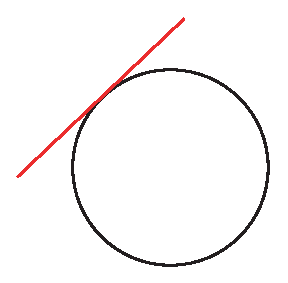
\includegraphics[height=3.39cm]{313.eps}
% napperon.eps : 300dpi, width=3.39cm, height=3.39cm, bb=0 0 400 400
    \end{center}
Therefore, the answer is d).\\

314-- A convex polygon has 8 sides. What is the sum of the size of its internal angles?\\

a) 1080$^{\circ}$\\
b) 1260$^{\circ}$\\
c) 1440$^{\circ}$\\
d) 1800$^{\circ}$\\


R\'eponse : a)\\

R\'etroaction : \\
A convex polygon with 8 sides can be decomposed into 6 triangles. We know that the sum of the sizes of the internal angles
of a triangle is 180$^{\circ}$. The find the sum of the sizes of the internal angles of a polygon with 8 sides, simply
compute $180^{\circ}\times6=1080^{\circ}$.\\
The answer is a).\\

315-- In a polygon, what is the sum of an exterior angle and its associated internal angle?\\

a) 45$^{\circ}$\\
b) 90$^{\circ}$\\
c) 180$^{\circ}$\\
d) 360$^{\circ}$\\

R\'eponse : c)\\

R\'etroaction : \\
By definition, an exterior angle and its associated internal angle
make a straight line, i.e. a flat angle.
The size of a flat angle is 180$^{\circ}$ and the answer is c).\\

316-- A window is shaped like a regular polygon and the sum of its internal angles is 1440$^{\circ}$. What is the shape of the window?\\

a) Decagon.\\
b) Dodecagon.\\
c) Hexagon. \\
d) Octagon.\\

R\'eponse : a)\\

R\'etroaction : \\
Let $s$ = sum of internal angles.\\
$n$ = number of sides of the window.\\[2mm]
We know that:\\[2mm]
$s = 180 \left( n-2\right). \\[2mm]
\frac{s}{180}=n-2\\[2mm]
\frac{s}{180}+2=n\\[2mm]
\frac{1440}{180}+2=10$\\[2mm]
Thus, the window has 10 sides. A regular polygon with 10 sides is called a decagon and the answer is a).\\

317-- How many extremities does a segment have?\\

a) 0\\
b) 1\\
c) 2\\
d) Infinitely many.\\

R\'eponse : c)\\

R\'etroaction : \\
A segment is finite. It has two extremities and the answer is c).\\

318-- What is the plane geometrical figure with the largest area for a fixed perimeter?\\

a) Square.\\
b) Circle.\\
c) Octagon.\\
d) Triangle.\\

R\'eponse : b)\\

R\'etroaction :\\
The circle has the greatest surface area. The answer is b).\\

319-- Achilles has a 12 m flexible band to fence his garden. Since Achilles is a little bit out there, his garden's shape does not matter to him. However, he wants to fence his garden with his flexible band in such a way that his garden has the largest area possible. What shape must his garden have?\\

a) Square.\\
b) Circle.\\
c) Pentagon.\\
d) Equilateral triangle.\\

R\'eponse : b)\\

R\'etroaction : \\
You don't need to compute anything! For a given perimeter, the circle is the plane figure with the largest area. Therefore, the answer is b).\\


320-- Which answer choice is the odd one out?\\

$4\longmapsto 360^{\circ}$\\
$5\longmapsto 540^{\circ}$\\
$7\longmapsto 920^{\circ}$\\
$8\longmapsto 1440^{\circ}$\\

a) The odd one out is $4\longmapsto 360^{\circ}$.\\
b) The odd one out is $5\longmapsto 540^{\circ}$.\\
c) The odd one out is $7\longmapsto 920^{\circ}$.\\
d) The odd one out is $8\longmapsto 1440^{\circ}$.\\

R\'eponse : c)\\

R\'etroaction : \\
The rule is $\left(n-2\right) \times 180$.\\
$\left( 7-2 \right) \times 180 = 5\times180=900\neq920$\\
Therefore, the answer is c).\\


322-- Which answer choice represents a random experiment?\\

a) The draw of a loto 6/49 number.\\
b) The roll of a loaded dice whose faces all present the number two.\\
c) Drawing a marble in a bag containing only blue marbles.\\
d) Drawing a card in a deck containing only aces of spade.\\

R\'eponse : a)\\

R\'etroaction :\\
A random experiment is an experiment whose result is completely random. The only answer choice that presents a random experiment is \og the draw of a loto 6/49 number\fg. Therefore, the answer is a).\\

323-- A particular random experiment consist in rolling a dice. What is the probability space?\\

a) $\Omega=\{7\}$\\
b) $\Omega=\{1, 2, 3, 4, 5, 6\}$\\
c) $\Omega=\{2, 3, 4, 5, 6\}$\\
d) $\Omega=\{$even, odd$\}$\\

R\'eponse : b)\\

R\'etroaction : \\
The probability space, represented by the symbol $\Omega$ (pronounced \emph{omega}), is the set of all possible results. When a dice is rolled, the possible outcomes are 1, 2, 3, 4, 5, and 6. Therefore, the answer is b).\\

324-- The probability space associated to a random experiment is represented by the symbol $\Omega$. How does this symbol read out?\\

a) Gamma.\\
b) Ohm.\\
c) Olala.\\
d) Omega.\\

R\'eponse : d)\\

R\'etroaction : \\
The symbol $\Omega$ is a Greek letter that is  pronounced \emph{omega}. The answer is d).\\

325-- A green and a red dice are rolled. How many possible results are there in this experiment?\\

a) 6\\
b) 12\\
c) 36\\
d) $46,656$\\

R\'eponse : c)\\

R\'etroaction : \\
This random experiments has two steps. Each step has 6 possible
outcomes. By the multiplication rule, there are
$6\times6=36$ possible results. Therefore, the answer is c).\\

326-- In a multi-step random experiment, the first step has $m$ possible results, the second step has $n$ possible results, the third step has $p$ possible results, the fourth step has $q$ possible results, $\ldots$, and the last step has $k$ possible results. What is the total number of possible results of this experiment?\\

a) $m+n+p+q+\ldots+k$\\
b) $m\times n\times p\times q\times \ldots \times k$\\
c) $m\times n\times p\times q\times k$\\
d) $m+n+p+q+k$\\

R\'eponse : b)\\

R\'etroaction : \\
This question exemplifies the conditions of application of the multiplication rule in probabilities. The answer is b).\\

327-- In a restaurant, the menu of the day offers soup, cheese sticks, or a vegetable juice for the appetizer, spaghetti,
 lasagna, or pizza for the entree, and ice cream or apple pie for dessert. How many different combinations of meals can be ordered with this menu?\\

a) 8\\
b) 12\\
c) 18\\
d) 27\\

R\'eponse : c)\\

R\'etroaction : \\
One must use the multiplication rule.\\
$3\times3\times2=18$\\
Therefore, the answer is c).\\


328-- How many two digit numbers are there in base 10?\\

R\'eponse : 90\\

R\'etroaction :\\
The two digit numbers are :\\

10, 11, 12, 13, 14, 15, 16, 17, 18, 19, \\
20, 21, 22, 23, 24, 25, 26, 27, 28, 29, \\
30, 31, 32, 33, 34, 35, 36, 37, 38, 39, \\
40, 41, 42, 43, 44, 45, 46, 47, 48, 49, \\
50, 51, 52, 53, 54, 55, 56, 57, 58, 59, \\
60, 61, 62, 63, 64, 65, 66, 67, 68, 69, \\
70, 71, 72, 73, 74, 75, 76, 77, 78, 79, \\
80, 81, 82, 83, 84, 85, 86, 87, 88, 89, \\
90, 91, 92, 93, 94, 95, 96, 97, 98, 99. \\

There is a way to find how many two digit numbers there are without
listing them all. Simply think about the multiplication rule. There
are 10 possible choices in the unit position, \emph{i.e.} 0, 1, 2,
3, 4, 5, 6, 7, 8, or 9. There are only 9 possible choices in the
tens' position because a
two digit number cannot start with 0. Therefore, there are $9\times10=90$ two digit numbers.\\

329-- How many three digit numbers are there in base 10?\\

a) 729\\
b) 900\\
c) 999\\
d) 1,000\\

R\'eponse : b)\\

R\'etroaction : \\
The three digit numbers are 100, 101, 102, 103, \ldots , 998, 999.
It is not necessary to list all of them to answer this question. Simply think about the multiplication rule. There are 10 possible choices in the units' position, i.e. 0, 1, 2, 3, 4, 5, 6, 7, 8 or 9. There are also 10 possible choices in the tens' position and the hundreds' position only has 9 possible choices because a three digit number cannot start with 0. Therefore, there are $9\times10\times10=900$ three digit numbers and the answer is b).\\


330-- How many 6 digit numbers are there in base 10?\\

a) $46,656$\\
b) $600,000$\\
c) $900,000$\\
d) $1,000,000$\\

R\'eponse : c)\\

R\'etroaction : \\
The 6 digit numbers are $100,000$,  $100,001$, $100,002$, \ldots
  $999,998$,  $999,999$. It is not necessary to list them all to find how many there are. Simply think about the multiplication rule.\\
There are 10 possible choices in the units' position, \emph{i.e.} 0,
1, 2, 3, 4, 5, 6, 7, 8 or 9. There are also 10 possible choices in
the tens', hundreds' thousands', and ten thousands' positions.
However, the hundred thousands' position only has 9 possible choices because a 6 digit number cannot start with 0. Therefore, the are $9\times10\times10\times10\times10\times10=900,000$ 6 digit numbers and the answer is c).\\


332-- In the \emph{three digit daily}, there are three plastic boxes
each containing balls numbered from 0 to 9. A single ball is drawn
out of each box.
How many possible results are there?\\

a) 30\\
b) 300\\
c) 900\\
d) 1,000\\

R\'eponse : d)\\

R\'etroaction : \\
One must think about the multiplication rule.\\
First box : 10 possible choices.\\
Second box : 10 possible choices.\\
Third box : 10 possible choices.\\
The multiplication rule says that the number of choices at each step must be multiplied.\\
$10\times10\times10=1,000$\\
Therefore, there are 1,000 possible results and the answer is d).\\

333-- Which answer choice correctly completes the following statement : \og In an equiprobable random experiment,  $\ldots$\fg ?\\

a) the first event has the highest probability to occur.\\
b) the last event has the highest probability to occur.\\
c) all the events have the same probability to occur.\\
d) the events don't all have the same probability to occur.\\

R\'eponse : c)\\

R\'etroaction : \\
The prefix\og equi\fg\ means equal. The events all have the same probability to occur. The answer is c).\\

334-- Out of the following four decimal numbers, which one may represent the probability of an event?\\

a) $-1.53$\\
b) $-0.53$\\
c) 0.53\\
d) 1.53\\

R\'eponse : c)\\

R\'etroaction : \\
The probability of an event is a number between 0 and 1 or
equal to 0 or 1. Therefore, the answer is c).\\

335-- Which answer choice correctly completes the following statement : \og The probability of an event is a number between $\ldots$  or equal to 0 or 1.\fg ?\\

a) 0 and 10\\
b) 0 and 1\\
c) 1 and 2\\
d) 1 and 10\\

R\'eponse : b)\\

R\'etroaction : \\
The probability of an event is a number between 0 and 1 or equal to 0 or 1. Therefore, the answer is b).\\

336-- In an ordinary 52 card deck, what is the probability to draw the ace of spade with a single draw?\\

a) $\frac{1}{52}$\\[2mm]
b) $\frac{4}{52}$\\[2mm]
c) $\frac{1}{13}$\\[2mm]
d) $\frac{1}{4}$\\

R\'eponse : a)\\

R\'etroaction : \\
A 52 card deck has a single ace of spade. Therefore, there is 1 chance out of 52 to draw it. The answer is a).\\

337-- Our of the four following fractions, which one can represent the probability of an event?\\

a) $\frac{9}{8}$\\[2mm]
b) $\frac{10}{9}$\\[2mm]
c) $\frac{2}{1}$\\[2mm]
d) $\frac{8}{8}$\\

R\'eponse : d)\\

R\'etroaction : \\
The probability of an event is a number between 0 and 1 or equal to 0 or 1.\\[2mm]
$\frac{8}{8}=1$\\[2mm]
Therefore, the answer is d).\\

338-- In an ordinary 52 card deck, what is the probability to draw a queen with a single draw?\\

a) $\frac{1}{52}$\\[2mm]
b) $\frac{1}{26}$\\[2mm]
c) $\frac{1}{13}$\\[2mm]
d) $\frac{1}{4}$\\

R\'eponse : c)\\

R\'etroaction : \\
An ordinary card deck contains 4 queens. Therefore, there are 4 chances out of 52 to draw a queen.\\[2mm]
$\frac{4}{52}=\frac{1}{13}$\\[2mm]
Thus, the answer is c).\\

339-- A letter of the word \og probability\fg. is picked out randomly. What is the probability of getting the letter a?\\

a) $\frac{1}{11}$\\[2mm]
b) $\frac{2}{11}$\\[2mm]
c) $\frac{2}{10}$\\[2mm]
d) $\frac{1}{10}$\\

R\'eponse : b)\\

R\'etroaction : \\
The word \og probability\fg  contains 11 letters, 2 of which are a's. Therefore, there are 2 chances out of 11 to get this letter.\\[2mm]
The answer is b).\\

340-- Garfield has just tossed a coin 7 times and it has landed on tail each time. Which statement correctly describes the situation for the eighth toss?\\

a) Garfield has just as many chances to get head or tail\\
b) It is more likely that Garfield gets head than tail.\\
c) It is more likely that Garfield gets tail than head.\\
d) It is less likely that Garfield gets tail than head.\\

R\'eponse : a)\\

R\'etroaction : \\
Each toss is independent. Garfield Garfield has just as many chances to get head or tail on any toss. The answer is a).\\


342-- A random experiment has 6 possible results. What is the sum of the probabilities of those 6 results?\\

a) 0.99\\
b) 1\\
c) 3 \\
d) 6\\

R\'eponse : b)\\

R\'etroaction : \\
The sum of the probabilities of the 6 possible results is 1. The answer is b).\\

343-- A random experiment has only three possible results. The probability of the first result is $\frac{3}{16}$ and the probability of the second result is $\frac{7}{16}$. What is the probability of the third result?\\

a) $\frac{10}{16}$\\[2mm]
b) $\frac{13}{16}$\\[2mm]
c) $\frac{9}{16}$\\[2mm]
d) $\frac{3}{8}$\\

R\'eponse : d)\\

R\'etroaction : \\
The sum of the probabilities of the first two results is:
$\frac{3}{16}+\frac{7}{16}=\frac{10}{16}$.\\[2mm]
The sum of the probabilities of the three results must be 1.\\[2mm]
Therefore, the probability of the third result is:
$1-\frac{10}{16}=\frac{16}{16}-\frac{10}{16}=\frac{6}{16}=\frac{3}{8}.$\\[2mm]
The answer is d).\\

344-- A game consist in tossing a coin and rolling a dice. What is the probabity to get the result (tail, 1)?\\

a) $\frac{1}{12}$\\[2mm]
b) $\frac{1}{8}$\\[2mm]
c) $\frac{1}{4}$\\[2mm]
d) $\frac{2}{3}$\\[2mm]

R\'eponse : a)\\

R\'etroaction : \\
In this random experiment, tossing the coin and rolling the dice are two independent events. The probability associated with the two events must be multiplied.
The probability to get tail on a coin's toss is $\frac{1}{2}$ and the probability to get 1 on a dice's roll is $\frac{1}{6}$.\\[2mm]
Since $\frac{1}{2}\times \frac{1}{6}=\frac{1}{12}$, the answer is a).\\

345-- Pinocchio's female hamster has four offsprings. What is the probability that all the offsprings are female?\\

a) $\frac{1}{32}$\\[2mm]
b) $\frac{1}{16}$\\[2mm]
c) $\frac{1}{8}$\\[2mm]
d) $\frac{1}{2}$\\

R\'eponse : b)\\

R\'etroaction : \\
Each new born hamster has 1 chance out of 2 to be a female, independently of the sex of its siblings. By multiplying the probability of the four events, we get:\\[2mm]
$\frac{1}{2}\times\frac{1}{2}\times\frac{1}{2}\times\frac{1}{2}=\frac{1}{16}$\\[2mm]
Therefore, the answer is b).\\

346-- The probability that a particular event happens is $p$. What is the probability that this event does not happen?\\

a) $2p$\\
b) $p$\\
c) $1-p$\\
d) $-p$\\

R\'eponse : c)\\

R\'etroaction : \\
The sum of the probabilities that the event happens and does not happen is 1.\\
Thus, we have P(happens) + P(does not happen) = 1\\
1 -- P(happens) = P(does not happen) \\
$1 - p$ = P(does not happen)\\
Thus, the probability that the event does not happen is $1-p$. The answer is c).\\

347-- A random experiment has 3 steps, wherein respectively P(F) =
$\frac{1}{a}$, P(3) = $\frac{1}{b}$, and P($\alpha$) = $\frac{1}{c}$. What is the probability to get the result(F, 3, $\alpha$)?\\

a) $\frac{1}{a+b+c}$\\[2mm]
b) $\frac{1}{abc}$\\[2mm]
c) $\frac{3}{a+b+c}$\\[2mm]
d) $\frac{3}{abc}$\\

R\'eponse : b)\\

R\'etroaction : \\
To probabilities of each event must ne multiplied.\\[2mm]
$\frac{1}{a}\times\frac{1}{b}\times\frac{1}{c}=\frac{1}{abc}$\\[2mm]
Therefore, the answer is b).\\

348-- What is the probability that Christmas happens on the 25$^{th}$ of December this year?\\

a) 0\\[2mm]
b) $\frac{1}{365}$\\[2mm]
c) $\frac{1}{31}$\\[2mm]
d) 1\\

R\'eponse : d)\\

R\'etroaction : \\
Christmas always happen on December 25! (it is a certain event).
Since the probability of a certain event is 1, the answer is d).\\

349-- In a 52 card deck, what is the probability of drawing an ace of spade and then an ace of diamond if the first drawn card is not put back in the deck?\\

a) $\frac{1}{2704}$\\[2mm]
b) $\frac{1}{2652}$\\[2mm]
c) $\frac{1}{104}$\\[2mm]
d) $\frac{1}{103}$\\

R\'eponse : b)\\

R\'etroaction : \\
The probability to get the ace of spade in the first draw is
$\frac{1}{52}$. The probability to get an ace of diamond in the
second draw is $\frac{1}{51}$, because the card first drawn has not
been put back in the deck. Therefore, the joint probability of
drawing an ace of spade followed by an ace of diamond is
$\frac{1}{52}\times\frac{1}{51}=
\frac{1}{2652}$.\\
The answer is b).\\

350-- Tintin has left his clean clothes basket in a basket in the basement. This basket contains 10 unpaired pairs of socks.
It is pitch-dark and Tintin randomly picks one sock, and then another. What is the probability that the two socks he has picked make a pair?\\

a) $\frac{1}{380}$\\[2mm]
b) $\frac{1}{39}$\\[2mm]
c) $\frac{1}{20}$\\[2mm]
d) $\frac{1}{19}$\\

R\'eponse : d)\\

R\'etroaction : \\
On his first draw, Tintin has a probability of 1 to draw a sock. On the second pick, there are only 19 socks left, one of which correctly pairing with the first pick. Thus, there is one chance out of 19 to pick it. The probability to pick a pair is $1\times\frac{1}{19}=\frac{1}{19}$. Therefore, the answer is d).\\




\end{document}
